\section{Exact numerator reduction with learned identity choices}
\label{sec:notes-tensor-results}
The preceding scalar recurrence accepts raised denominator powers. A polynomial numerator can prevent that path from applying, even when only one loop needs reduction. We extend the exact stage to such numerators by resolving the loop momentum into directions parallel and perpendicular to the external vectors seen by the denominators. Angular averages remove the perpendicular numerator factors, after which the scalar recurrence lowers the remaining powers. Tensor reduction and general one-loop generating functions provide the established context~\cite{DennerDittmaier2006,Hu2025}; Appendix~\ref{app:notes-tensor-reduction} derives the specific angular and signed-index IBP identities used here.

There are two useful orders for these identities. We can remove the numerator before lowering raised propagator powers, or use the signed-index IBP relation to lower those powers first. In either order, the calculation ends at unit-power scalar sectors. The model selects this order and whether to lower the largest or smallest raised positive power. The implementation shares intermediate reductions within each request and reuses identical independent components within that request. Its four actions therefore change the path through exact identities. Exact arithmetic supplies every reduction coefficient. We keep the preceding native seed model for inputs that still require Kira.

We also use the derived denominator structure to simplify the exact arithmetic. Every dimension-dependent denominator is a product of factors $d+j$ with integer $j$. Keeping these factors explicit permits exact cancellation by polynomial division, as derived in Eqs.~\eqref{eq:notes-tensor-factored-field}--\eqref{eq:notes-tensor-factored-add}. The final model learns from complete timings with this arithmetic in place. A fixed-action control uses the same arithmetic, so that the measured effect of the model remains separate from the exact improvement.

\subsection{Families, checks, and comparison design}
The new one-loop families contain two, three, or four physical denominators and one or two auxiliary coordinates, with at most five coordinates in total. Numerator rank means $\sum_j\max(-a_j,0)$, and excess positive power means $\sum_j\max(a_j-1,0)$. The training requests span numerator ranks one through four and excess powers zero through three. They use distinct rational masses and off-shell scalar products, with symbolic $d$. Appendix~\ref{app:notes-tensor-reduction} specifies the construction and the wider implementation bounds. These are reductions at rational kinematic points; they do not reconstruct a general symbolic multiscale answer.

We measure all four actions on 24 training requests and 12 separate validation requests. Their mass and scalar-product profiles differ across splits, although some index patterns recur. The final test changes both the profiles and target batches. Sixteen requests use the massive training structures, four further requests use massless or mixed-mass sectors, and twelve requests use independent products of tensor bubbles at each loop order from two through thirteen. Eight new native requests test the retained seed model in planar and nonplanar massless two-loop boxes, while four vacuum-tree requests check that the preceding exact path still works. The products establish a factorized high-loop extension. Each method returns the product of component reductions, so the timed output retains the factors instead of expanding every product of master integrals. These requests do not test a coupled thirteen-loop scattering reduction.

The development checks compare 44 exact coefficients with native Kira in six requests, test 37 coefficients in independently assembled signed IBP residuals, and test changes of loop names, loop signs, and propagator order. The final arithmetic passes 240 rational-function comparisons and repeats the native pilot agreement. Every new training and validation output is compared with the first symbolic-field implementation. The reserved tensor results are checked through the alternate recurrence, while native box results use separately prepared Kira references. If a native result uses a different basis, the external check reduces that basis before comparing coefficients. These checks follow the algebra of the reduction and do not replace the derivation.

Each reserved application starts in a fresh process and runs three times, with method order rotated on the same worker. The eighteen-second limit applies to every timed method. Total time includes input reading, recognition, model loading and prediction, exact algebra or native recovery, output, and exit. The separate reference calculation and external coefficient comparison lie outside all application timers. The preceding native method uses its existing master-index registry. A failed request remains in the completion counts and receives no finite speed factor. We sum per-request median times only for requests that both methods complete and verify in all three repetitions. The resampling interval uses the request-level procedure of the request-resampling calculation defined at the end of the final-results subsection below.

\subsection{Final exact and learned results}
Validation selects 1 cost tree, depth at most 1, minimum leaf population 2, and a predicted-saving margin of 8\%. The fixed control removes the numerator first and then lowers the smallest raised positive power. The validation rule disables the new learned choice. Its validation cost, including a one-millisecond allowance per request, is 3.207 seconds, against 3.195 seconds for the fixed choice. These values determine deployment; the final test supplies the independent timing result.

The deployment rule leaves the tensor model disabled. Its final application and fixed control therefore use the same action; their timing difference measures run variation. The retained native seed model remains active on its eligible requests.

\begin{table}[!htbp]\centering\small
\caption{Final complete-time comparisons. Counts give control/final completions, and times sum medians on matched completed requests. The first tensor implementation uses a general rational-function field. The fixed control uses the final exact arithmetic with the relevant learned choice disabled. All entries are measurements of this study.}
\label{tab:notes-tensor-results}
\begin{tabularx}{\linewidth}{@{}Yrrrr@{}}\toprule
Comparison & Done & Paired & Control (s) & Final (s)\\\midrule
Tensor / preceding application & 20/20 & 20 & 53.518 & 6.343 \\
Tensor / first implementation & 20/20 & 20 & 26.703 & 6.343 \\
Independent products / preceding & 12/12 & 12 & 121.891 & 3.006 \\
Native boxes / fixed seed choice & 8/8 & 8 & 53.468 & 51.894 \\
Native boxes / preceding & 8/8 & 8 & 50.717 & 51.894 \\
All 44 requests / preceding & 44/44 & 44 & 227.011 & 62.225 \\
Vacuum regression / preceding & 4/4 & 4 & 0.885 & 0.982 \\
\bottomrule\end{tabularx}\end{table}

\begin{table}[!htbp]\centering\small
\caption{Physical scope of the final one-loop tensor comparison. Times sum matched request medians against the preceding application. Mass classes with a single request have evidence from that case alone.}
\label{tab:notes-tensor-types}
\begin{tabularx}{\linewidth}{@{}Yrrr@{}}\toprule
Integral class & Paired & Preceding (s) & Final (s)\\\midrule
Massive bubbles & 8 & 13.833 & 1.911 \\
Massive triangles & 4 & 9.020 & 1.291 \\
Massive boxes & 4 & 20.998 & 2.185 \\
Massless bubble & 1 & 1.409 & 0.212 \\
Mixed-mass bubble & 1 & 1.694 & 0.183 \\
Mixed-mass triangle & 1 & 1.981 & 0.270 \\
Mixed-mass box & 1 & 4.583 & 0.290 \\
\bottomrule\end{tabularx}\end{table}\FloatBarrier

The tensor comparison with the preceding application gives time ratio 0.119, with a central 95\% request-resampling interval of $[0.106,0.133]$. The final method is slower on 0 of 20 matched requests.

The tensor comparison with the first implementation gives time ratio 0.238, with a central 95\% request-resampling interval of $[0.214,0.262]$. The final method is slower on 0 of 20 matched requests.

The retained native seed model against fixed choices gives time ratio 0.971, with a central 95\% request-resampling interval of $[0.936,1.011]$. The final method is slower on 2 of 8 matched requests. The interval includes equal time, so this sample does not resolve a consistent gain across its requests.

The final application completes 44 of 44 requests in every repetition, with 13,272 coefficient comparisons across the timed methods. The new tensor selector makes no predictions because validation retains the fixed action. The retained seed model is evaluated on 8 of the eight native requests. The complete-time gains against the preceding application include the new exact identities and arithmetic; the native fixed control measures the extra learned choice.

Across all 44 requests, total time changes from 227.011 to 62.225 seconds, or 72.6\% less time on this collection. The final application is slower on 10 requests. The native requests take 1.023 times the preceding application's time, and the four retained vacuum requests take 1.110 times its time. These regressions remain in the overall result; the new exact tensor path supplies the large saving.

\begin{figure}[!htbp]\centering
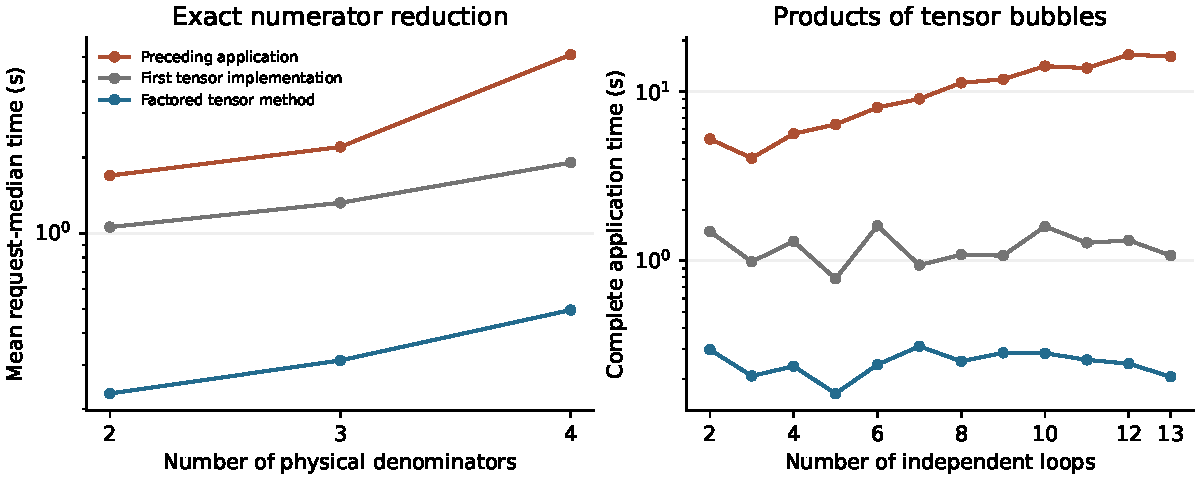
\includegraphics[width=\linewidth]{paper_figures/tensor_reduction.pdf}
\caption{Exact numerator reduction and factored dimension denominators reduce complete time on the plotted requests. The left panel averages the request medians, on common completed requests, for each physical-denominator count. The right panel shows independent tensor-bubble products through thirteen loops. Only requests completed in all repetitions appear; missing points represent incomplete controls. The logarithmic time axes show the full measured range. The fixed-control comparisons in Table~\ref{tab:notes-tensor-results} separately measure the learned contribution.}
\label{fig:notes-tensor-results}
\end{figure}
\FloatBarrier

The added exact domain covers rational one-loop numerator reductions and their independent products under the stated matrix and power conditions. The retained vacuum and massless tree identities supply further connected high-loop domains. General symbolic multiscale kinematics, singular tensor projections requiring other identities, and arbitrary coupled high-loop scattering remain outside this extension. The results establish the measured savings and their limits; they do not establish a globally shortest reduction path.

For each comparison, we resample its matched requests with replacement 2,000 times, sum the request medians in each resample, and divide the final sum by the control sum. The reported central interval uses the 2.5 and 97.5 percent quantiles of these ratios. This describes variation across the finite request collection.
\subsection{First tensor implementation and preliminary comparison}
For native, the first implementation completes 8 of 8 requests in all repetitions. Its preceding control completes 8. On 8 matched requests, the control and first tensor times are 43.859 and 43.616 seconds.
For other masses, the first implementation completes 4 of 4 requests in all repetitions. Its preceding control completes 4. On 4 matched requests, the control and first tensor times are 8.917 and 4.174 seconds.
For previous exact, the first implementation completes 4 of 4 requests in all repetitions. Its preceding control completes 4. On 4 matched requests, the control and first tensor times are 0.881 and 1.015 seconds.
For products, the first implementation completes 12 of 12 requests in all repetitions. Its preceding control completes 11. On 11 matched requests, the control and first tensor times are 111.212 and 12.690 seconds.
For tensor, the first implementation completes 16 of 16 requests in all repetitions. Its preceding control completes 16. On 16 matched requests, the control and first tensor times are 61.705 and 21.466 seconds.
The first identity-order model gives ratio 1.065 against its fixed action, with request interval $[1.039,1.097]$. Its weights remain stored, while the final arithmetic uses a separately trained policy.
The preliminary fixed-control measurement for the three-loop product contains a startup import failure during a source transfer. The outcome remains in the saved record and is excluded from completed-time comparisons. Subsequent transfers retain unchanged files and replace changed sources atomically. The final comparison uses a new collection and preserves all failures separately.
